%----------------------------------------------------------------------------------------
  %	PACKAGES AND OTHER DOCUMENT CONFIGURATIONS
  %----------------------------------------------------------------------------------------
  
  % \documentclass[twoside,twocolumn]{article}
  \documentclass[oneside,onecolumn]{article}
  \usepackage{ctex}
  \usepackage{blindtext} % Package to generate dummy text throughout this template 
  
  \usepackage{amsmath,amsthm,amsfonts,amssymb,bm}
  \usepackage{mathptmx}
  
  %%\usepackage[sc]{mathpazo} % Use the Palatino font
  \usepackage[T1]{fontenc} % Use 8-bit encoding that has 256 glyphs
  \linespread{1.05} % Line spacing - Palatino needs more space between lines
  \usepackage{microtype} % Slightly tweak font spacing for aesthetics
  
  \usepackage[english]{babel} % Language hyphenation and typographical rules
  
  \usepackage[hmarginratio=1:1,columnsep=20pt]{geometry} % Document margins
  \geometry{a4paper,scale=0.8}
  \usepackage[small,labelfont=bf,up,textfont=it,up]{caption} % Custom captions under/above floats in tables or figures
  \usepackage{booktabs} % Horizontal rules in tables
  
  \usepackage{lettrine} % The lettrine is the first enlarged letter at the beginning of the text
  
  \usepackage{enumitem} % Customized lists
  \setlist[itemize]{noitemsep} % Make itemize lists more compact
  
  \usepackage{abstract} % Allows abstract customization
  \renewcommand{\abstractnamefont}{\normalfont\bfseries} % Set the "Abstract" text to bold
  \renewcommand{\abstracttextfont}{\normalfont\small\itshape} % Set the abstract itself to small italic text
  
  \usepackage{titlesec} % Allows customization of titles
  \renewcommand\thesection{\arabic{section}} % arabic numerals for the sections
  \renewcommand{\thesubsection}{\thesection.\arabic{subsection}}
  
  \titleformat{\section}[block]{\large\scshape\centering}{\thesection.}{1em}{} % Change the look of the section titles
  % \titleformat{\subsection}[block]{\large}{\thesubsection.}{1em}{} % Change the look of the section titles
  \titleformat{\subsection}[block]{\large\scshape}{\thesubsection.}{1em}{} % Change the look of the section titles
  
  \usepackage{fancyhdr} % Headers and footers
  \pagestyle{fancy} % All pages have headers and footers
  \fancyhf{} % Clear default header and footer
  \fancyfoot[C]{\thepage} % Add page number to the center of the footer
  \renewcommand{\headrulewidth}{0pt}
  
  \usepackage{titling} % Customizing the title section
  \date{}
  
  \usepackage[svgnames]{xcolor} % added by Wenyin for color
  % \usepackage{hyperref} % For hyperlinks in the PDF
  \usepackage[colorlinks=true,linkcolor=Maroon,anchorcolor=blue,citecolor=RoyalBlue,filecolor=blue,menucolor=blue,runcolor=blue,urlcolor=DodgerBlue]{hyperref} % For hyperlinks in the PDF
  
  % for multiple references with dash
  \usepackage[noadjust]{cite}
  \renewcommand{\citedash}{--}    % when \usepackage{cite}
  
  \usepackage{graphicx}
  \usepackage[export]{adjustbox}
  \graphicspath{ {./images/} }
  
  \usepackage{amsmath}
  \usepackage{amsfonts}
  \usepackage{amssymb}
  \usepackage{mathrsfs} % for \mathscr
  \usepackage{booktabs}
  \usepackage{multirow}
  
  \usepackage[T1]{fontenc}
  % To use \mdutchcal{ } as \mathcal of package dutchcal, the following commands are needed, from https://imathworks.com/tex/tex-latex-new-locally-defined-mathcal-font-for-math-equations/
  % Based on the code from mathalpha.sty: 
  \DeclareFontFamily{U}{dutchcal}{\skewchar \font =45}
  \DeclareFontShape{U}{dutchcal}{m}{n}{
  	<-> dutchcal-r}{}
  \DeclareFontShape{U}{dutchcal}{b}{n}{
  	<-> dutchcal-b}{}
  \DeclareMathAlphabet{\mdutchcal}{U}{dutchcal}{m}{n}
  \SetMathAlphabet{\mdutchcal}{bold}{U}{dutchcal}{b}{n}
  \DeclareMathAlphabet{\mdutchbcal} {U}{dutchcal}{b}{n}
  
  % \usepackage{unicode-math} % for bold math font
  % \setmathfont{XITS Math}
  
  % vector, matrix and tensor
  % \newcommand{\vect}[1]{\boldsymbol{#1}}
  % \newcommand{\vect}{\symbf}
  % \newcommand{\vect}{\mathbf} % works for English letters but not for Greek letters 
  \newcommand{\vect}[1]{\mathbf{\boldsymbol{#1}}} % works for both English and Greek letters, but it does not work with mathtime pro lite fonts, see https://tex.stackexchange.com/questions/3535/bold-math-automatic-choice-between-mathbf-and-boldsymbol-for-latin-and-greek 
  % \newcommand{\matr}[1]{\boldsymbol{\mathrm{#1}}} % \matrix is defined in LaTeX2e kernel
  \newcommand{\tens}[1]{\boldsymbol{\mathrm{#1}}}
  
  \usepackage{mathtools} % for $\intertext{text}$
  
  % for footnote without number, from https://tex.stackexchange.com/questions/170511/footnotes-without-numbering
  \let\svthefootnote\thefootnote
  % \textheight 1in
  \newcommand\blankfootnote[1]{%
  	\let\thefootnote\relax\footnotetext{#1}%
  	\let\thefootnote\svthefootnote%
  }
  \let\svfootnote\footnote
  \renewcommand\footnote[2][?]{%
  	\if\relax#1\relax%
  	\blankfootnote{#2}%
  	\else%
  	\if?#1\svfootnote{#2}\else\svfootnote[#1]{#2}\fi%
  	\fi
  }
  
  %----------------------------------------------------------------------------------------
  %	TITLE SECTION
  %----------------------------------------------------------------------------------------
  
  \setlength{\droptitle}{-4\baselineskip} % Move the title up
  
  \pretitle{\begin{center}\Huge\bfseries} % Article title formatting
  	\posttitle{\end{center}} % Article title closing formatting
  \title{Multiscale Chirping Modes Driven by Thermal Ions in a Plasma with Reactor-Relevant Ion Temperature}
  \author{Author1, Author2}
  \renewcommand{\maketitlehookd}{%
  	\begin{abstract}
 在DIII-D托卡马克中,观测到了一种热离子驱动的爆发不稳定性,其快速频率啁啾可视为阿尔文离子温度梯度模式。该模式可以在从宏观设备尺寸到微湍流尺寸的广泛空间范围内被激发,并且扰动能量跨越多个空间尺度传播。径向模式结构能够在约$0.1\mathrm{~ms}$内从局部扩展到全局,并在等离子体边缘引起磁拓扑变化,这可能导致轻微干扰事件。由于该模式通常在高离子温度($\gtrsim 10 \mathrm{keV}$)和高-$\beta$等离子体区域内被观测到,因此未来反应堆中该模式的表现应进行研究,如有必要,应制定缓解策略。这是关于由于反应堆相关离子温度导致阿尔文连续体解稳定化的首次观测。
  	\end{abstract}
  }
  
  %----------------------------------------------------------------------------------------
  
  \begin{document}
  \begin{sloppypar}
  % Print the title
  \maketitle
 
 一个热核托卡马克反应堆需要离子温度$T_{i}\gtrsim10\mathrm{keV}$才能实现自持,需要大的$\beta$(等离子体与磁压力的比值)才能经济高效,需要避免破裂才能实现可靠,本文中我们描述了一种在高$T_{i}$的DIII-D等离子体中观察到的不稳定性,这可能会危及这些条件的可持续和同时实现。与电静能离子温度梯度驱动(ITG)湍流 [1] 不同,这种不稳定性的频谱由许多从 $n=1$ 至 $>21$ 的不同相干峰组成的软X射线电子密度下降的频域结构。尽管先前在高$T_{i}$下观察到类似的波数谱 [2],但这些模式的频率脉动很快,而且在高$\beta$下(即规范化 $\beta_{N} \sim 2.5$)被强烈地不稳定化。众所周知,啁啾模式是通过粒子之间的波粒共振相互作用来驱动能量粒子的,这可能会威胁到聚变反应堆中$\alpha$粒子的良好约束。然而,这里研究的啁啾模式是由反应堆所需的具有高$T_{i}$的热粒子的共振相互作用驱动的,这意味着在聚变反应堆中高温等离子体的操作面临着新的挑战。这种不稳定性经常触发重新连接,从而导致小型的破裂事件,并且在理想磁流体动力学(MHD)理论设定的$\beta$极限的一小部分处不稳定,从而危及经济反应堆的运行。这种危险的不稳定性具有由理论预测的电磁 Alfven ITG(AITG)[4-6] 的许多特性,并且与线性陀螺动力学不稳定性分析[7]一致。与先前在电阻等离子体中声称的 $ T_{i}\leq 0.75\mathrm{keV}$,没有检测到磁波扰动 $\tilde{b}$ 的AITG不同,这种观察到的模式,被认为是AITG,是多尺度的,具有相当的 $\tilde{b}$,并由$T_{i}>10 \mathrm{keV}$的热粒子驱动。
  
 该实验在一个低单空间单零点截面、$80 \mathrm{kV}$ 的氘束加热等离子体中进行,注入功率为$\sim 7 \mathrm{MW}$。托卡马克磁场强度为$2.1 \mathrm{~T}$,等离子体电流$I_{p}$为$1.6 \mathrm{MA}$。磁安全因子$q$的分布从磁轴处的$\sim 0.7$单调地增加至靠近等离子体边界的$\sim 4$。等离子体的约束性能优秀,$H_{98}$因子高达$\sim 2.5$,形成$T_{i} \sim 15 \mathrm{keV}$的热等离子体核心[9]。可以常规观测到具有快速下行的频率啁啾现象,如图1(a)所示。波沿离子弱磁方向涡向传播,并且沿等离子体电流方向在托卡马克方向传播。该模式在等离子体参考系中的实际频率约为$\sim 18 \mathrm{kHz}$,与$rational~surface~of~the~q=1$上的离子弱磁漂移频率$\omega_{i}^{*}$可比。该频率在不到$<3 \mathrm{~ms}$的时间内快速下行到接近$0 \mathrm{kHz}$,即实验室参考系中的多普勒频率。发现激发啁啾模式与$T_{i}$的变化非常敏感。例如,如图1(b)中的第178941次射线,尽管等离子体密度、平衡和中性束加热的情况与图1(c)中的第178943次射线相符,但啁啾模式几乎不可观测。而主要的差异在于所测得的$T_{i}$,当时未发现该啁啾模式时它比现在低$\sim 30 \%$,如图1(d)所示。有趣的是,在低$T_{i}$射线中,连续振荡模式变得更为突出,而模式动态的暂时转换也可以看到,如图1(b)中的箭头所示。
  
  \begin{figure}[htbp]
  	\centering
  	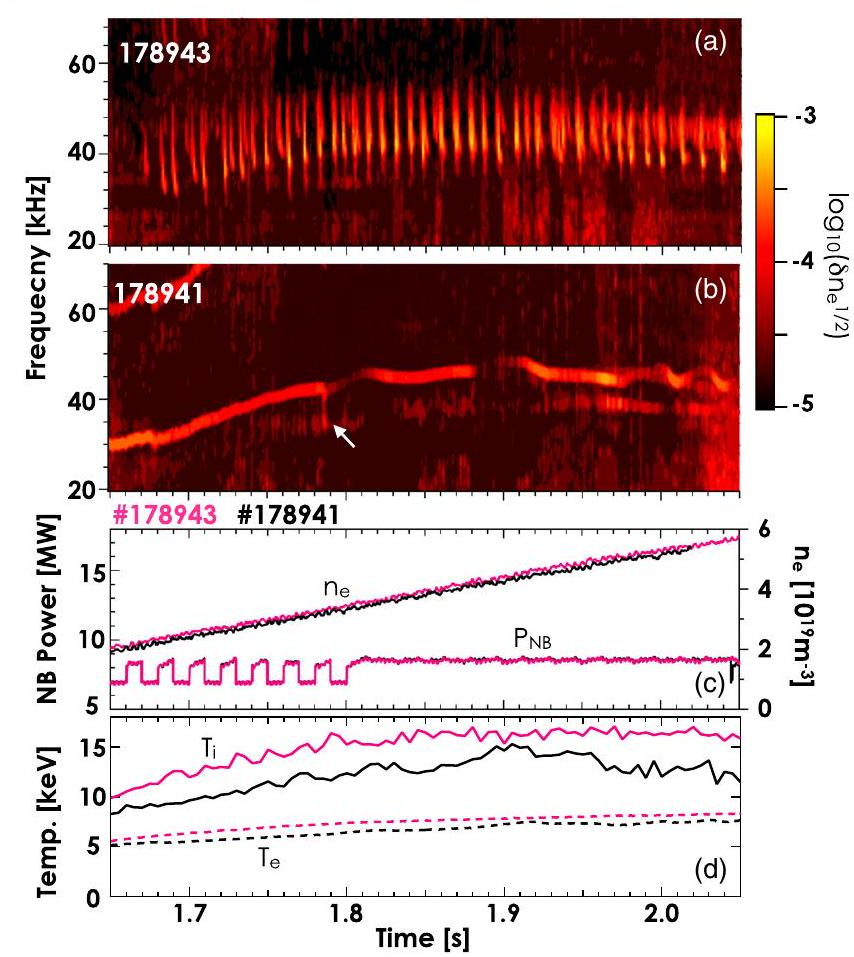
\includegraphics[max width=0.6\textwidth,max height=1.0\textheight]{2023_06_19_f8dbb752866ca158c73eg-2(1)}
  	\caption{Frequency spectra of the density fluctuations for shot No. 178943 and No. 178941 are shown in (a) and (b), respectively. The time evolutions of the line-averaged plasma density and neutral beam power in (c) and ion temperature (solid line) and electron temperature (dashed line) near the magnetic axis in (d) for shot No. 178943 (red) and No. 178941 (black).}
  	\label{figure1}
  \end{figure}
  
  
 Chirping模式的振幅对于相同的$T_{i}$,与快离子$\beta_{f}$呈反比例关系。图1(a)显示,当线平均等离子体密度几乎翻倍时(从$1.8 \mathrm{~s}$到$2.05 \mathrm{~s}$保持固定的中性束功率),振幅得到增强,即$\beta_{f}$下降了$>30 \%$ ,由TRANSP代码$[10,11]$估算。对于包含图2(a)中$>200$统计学分析的数据,也表明当存储式快离子能量的近似值$\left(P_{\mathrm{nb}} / n_{e}\right)$低而$T_{i}$高时,具有更大振幅的Chirping模式很有可能发生。在此,数据库中$P_{\mathrm{nb}} / n_{e}$的变化主要反映了等离子体密度的改变,因为高$T_{i}$是由于强烈的中性束功率维持的。其$\beta_{f}$的反比例依赖于粒子能量模式相反,后者在$\beta_{f}$超过一定阈值时被激发[12]。在图2(c)中,对于34个随机抽取的突发情况[见图2(b)]中的中子通量的时间导数进行了条件平均。结果如图2(c)的虚线所示。每个爆发在整个时间内中子速率几乎保持不变。此外,TRANSP NUBEAM代码[13]使用测量的等离子体轮廓预测的中子速率与检测到的中子通量相匹配,表明不会发生大量的核心快离子损失或重分布。应当指出,在这种高$T_{i}$等离子体条件下,TRANSP预测的热核反应中子产额与粒子束-目标反应中子产额是可比较的,例如在$1.9 \mathrm{~s}$时,分别为$2.25 \times 10^{15} \mathrm{~N} / \mathrm{s}$和$2 \times 10^{15} \mathrm{~N} / \mathrm{s}$。因此,如果有的话,对于$\leq 4 \%$的粒子束-目标中子产额变化,中子系统可能对于$\sim 2 \%$的系统检测限制不敏感。
  \begin{figure}[htbp]
  	\centering
  	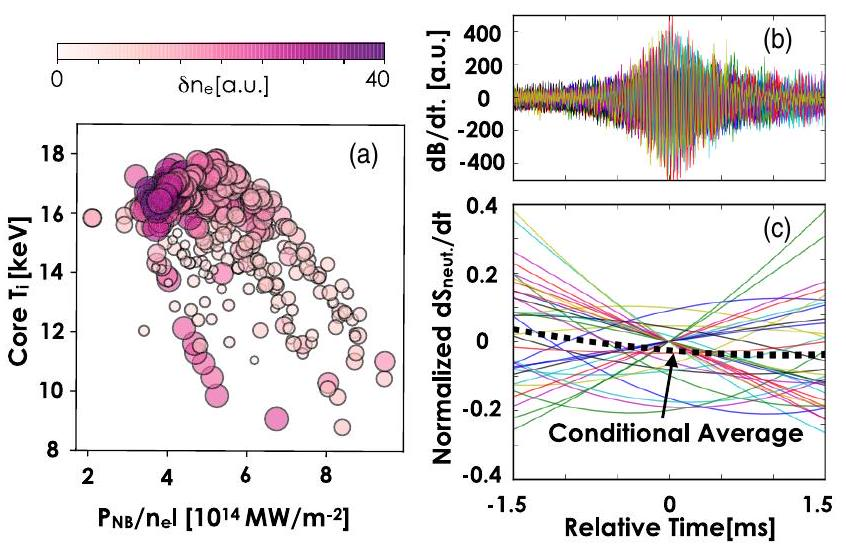
\includegraphics[max width=0.6\textwidth,max height=1.0\textheight]{2023_06_19_f8dbb752866ca158c73eg-2}
  	\caption{(a) Dependence of chirping mode amplitude on the neutral beam power normalized by the electron density $\left(\propto \beta_{f}\right)$ and the core $T_{i}$. The magnetic perturbations of 34 randomly sampled bursts (b) and corresponding time derivative of the neutron flux (c) are overlaid. The conditional averaged $d S_{\text {neut }} / d t$ is given as the dashed line in (c).}
  	\label{figure2}
  \end{figure}
  
  
 在毫秒时间尺度上频率啁啾和幅度爆发的特征通常是高能粒子驱动的不稳定性的标志。理论上,这是通过"相位锁定"过程来解释的,即波频率适应与高能粒子的共振条件以最大化模式驱动力[14]。相比之下,这里的数据表明,散体离子在激发啁啾模式中发挥了至关重要的作用。由于离子朗道阻尼对$T_{i}$的指数灵敏度[15],强烈的$T_{i}$依赖性表明,啁啾模式是由散体离子及其空间梯度激发的。
  
 多通道毫米波反射法[16]和磁探针测量等离子体边界“啁啾”模式激发的局部密度涨落$\tilde{n}_{e}$和磁扰动$\tilde{b}_{\theta}$,表明此类模式在$40\mathrm{kHz}$到$1\mathrm{MHz}$的广泛模频范围内被激发。磁学数据[17]显示,两个最低频率波的环向模数分别为1和2。由于这些模式出现于$q=1$磁通面上,因此推断其极向和环向模数为$(m, n)=(1,1)$到$(21,21)$[见图3(a)]。该失稳估计的波长范围从宏观MHD尺度到热离子回旋半径尺度$\rho_{i}$,相应的规范极向波数为$0.03<k_{\theta}\rho_{i}<0.6$,对应于局部的$T_{i}\sim12\mathrm{keV}$。上限与通常波数为$0.2<k_{\theta}\rho_{i}<0.5$的ITG相似[18]。模式行为的有趣细节总结如下:(1)在每次爆发前,图3(a)中介于$k_{\theta}$范围的显著$\tilde{n}_{e}$和$\tilde{b}_{\theta}$振幅,如图中箭头所示,作短暂不稳定,图3(a)和图3(b)中圆圈所示。阶梯状频谱中的峰对峰频率间隔为$32\mathrm{kHz}$,接近最低$k_{\theta}$波“啁啾”结束时的频率,即$31.5\mathrm{kHz}$。这表明爆发机制可能与谐振波波耦合通过多尺度扰动能量传递相关。(2) 在爆发的前半段,对应着快速的频率“啁啾”周期,检测到$\tilde{b}_{\theta}$的广泛$k_{\theta}$范围,但没有检测到明显$\tilde{n}_{e}$。但在爆发的后半段,对应着固定频率期间,高$k_{\theta}$波的$\tilde{b}_{\theta}$突然减小,$\tilde{n}_{e}$显著增强。在图3中,虚线标出了从主导的$\tilde{b}_{\theta}$到$\tilde{n}_{e}$的过渡。在少数情况下,高$k_{\theta}$范围内的$\tilde{b}_{\theta}$不存在,而$\tilde{n}_{e}$的类似时间迹象在广泛的小半径范围内都可以观察到,因此不是局部测量效应所致。
  \begin{figure}[htbp]
  	\centering
  	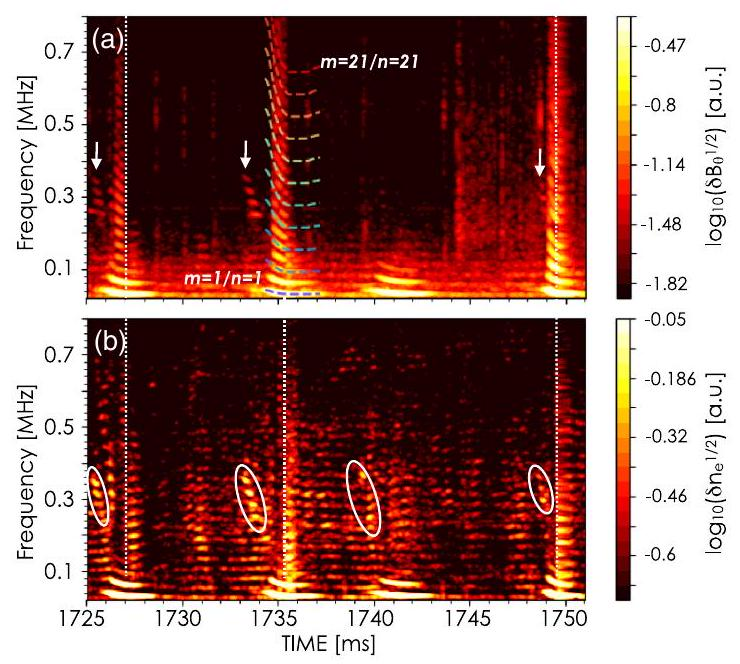
\includegraphics[max width=0.6\textwidth,max height=1.0\textheight]{2023_06_19_f8dbb752866ca158c73eg-3(1)}
  	\caption{Frequency spectra of the magnetic fluctuation at the plasma boundary (a) and density fluctuation spectra around the $q=1$ flux surface (b) in shot No. 178942 .}
  	\label{figure3}
  \end{figure}
  
  
 观察到的高 $k_{\theta}$ 波不是快速傅里叶变换作用于扭曲波形的人为效应。高 $k_{\theta}$ 波是真实存在的,因为高 $k_{\theta}$ 波独立于最低 $k_{\theta}$ 波。在中等 $k_{\theta}$ 范围内的 $\tilde{n}_e$ 扰动也在爆发之间处于边缘不稳定状态,通常在爆发之后立即稳定,例如在图3(b)的 $1728\mathrm{~ms}$ 处。根据理论,模式的多尺度激发可能是由非线性波波耦合引起的,称为成对交互级联[19]。还有可能是非线性耦合通过波粒子相互作用进行[20]。澄清非线性激发机制需要进一步的实验努力,留待将来的研究。
  \begin{figure}[htbp]
  	\centering
  	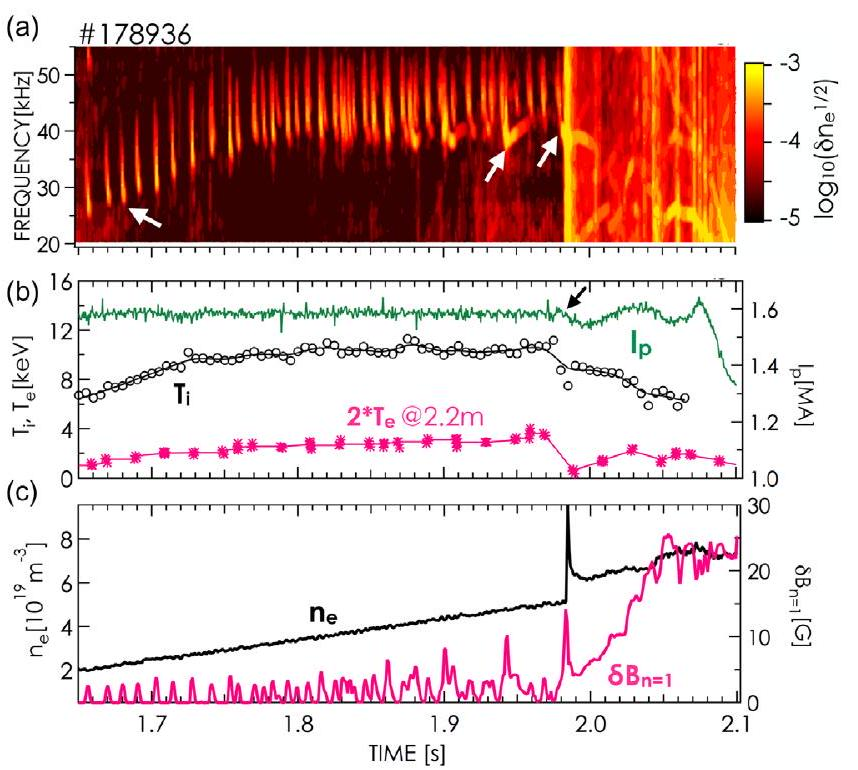
\includegraphics[max width=0.6\textwidth,max height=1.0\textheight]{2023_06_19_f8dbb752866ca158c73eg-3}
  	\caption{(a) Frequency spectra of density fluctuation measured by a $\mathrm{CO}_{2}$ interferometer. Time evolution of plasma current, ion temperature near the $q=1$ flux surface and electron temperature at $R=2.2 \mathrm{~m}$ in (b), volume-averaged electron density and integrated magnetic fluctuation of $n=1$ in (c).}
  	\label{figure4}
  \end{figure}
  
  
 “鸣叫模式可能对中子产生的影响是良性的,但在短时间的专门实验中会导致少数次轻微的干扰事件。图4显示,在频率升降音后,当$t\sim 1.9837 \mathrm{~s}$时,适中的$I_p$峰值[见图4(b)的箭头]伴随着实质性的密度增加。$I_p$峰值表明电流分布的重分布,通常被表征为干扰事件。密度峰值暗示来自第一壁的大量内向杂质通量。请注意,在该事件中,等离子体$\beta_N$约为2.7,远低于理想的$\beta_N$极限。”
  
 为了理解为什么某些啁啾模式会引起次要扰动事件而其他模式不会,我们比较了图4(a)中三个啁啾模式的径向模式结构,这三个模式用三个箭头表示。图5显示了用电子回旋辐射测量到的电子温度扰动$\tilde{T}_{e}$轮廓的时间演化。磁场扰动可作为参考。在$t\sim1.685\mathrm{~s}$时,爆发幅度相对较低。观察到的$\tilde{T}_{e}$本地化在$q=1$磁面,$R\sim1.9\mathrm{~m}$处,径向模式宽度约为$\sim 10 \mathrm{~cm}$,如图5(a)所示。径向方向上的相差几乎为零,即整个爆发过程中kink两性获得保持。
  \begin{figure}[htbp]
  	\centering
  	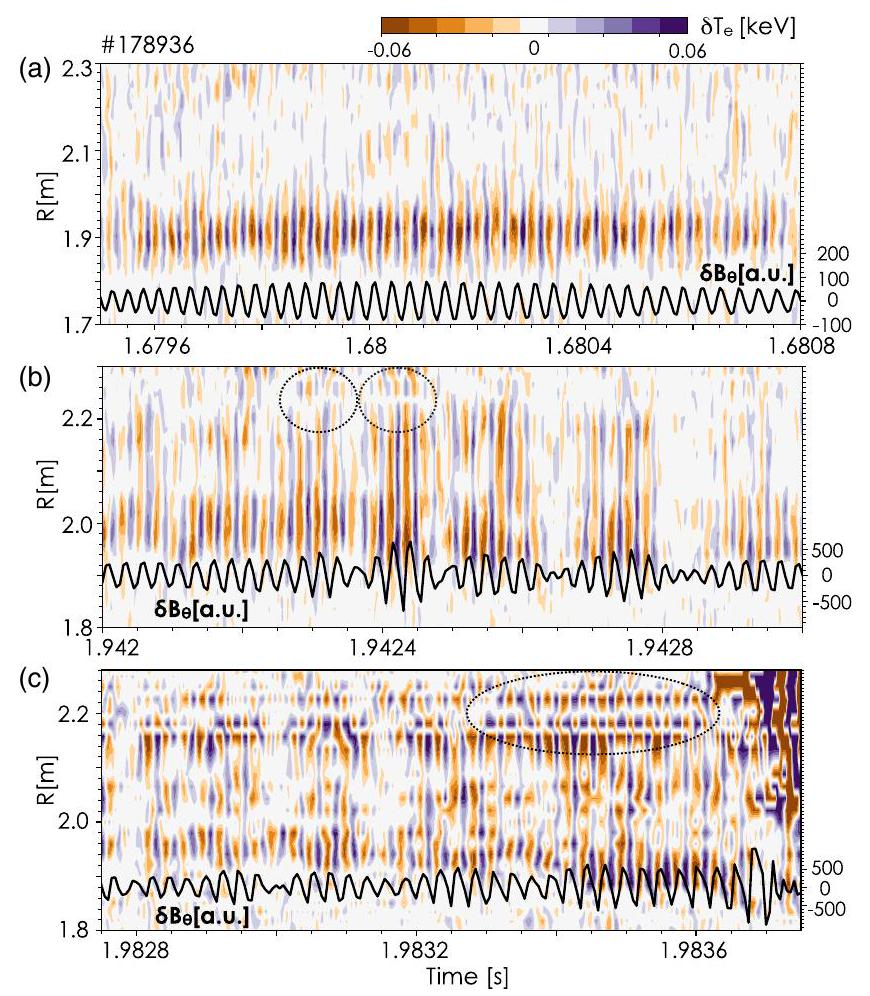
\includegraphics[max width=0.6\textwidth,max height=1.0\textheight]{2023_06_19_f8dbb752866ca158c73eg-4}
  	\caption{Time evolutions of the electron temperature fluctuations of the three chirping modes [marked by the three arrows in Fig. 4(a)] at $\sim 1.678 \mathrm{~s}, \sim 1.942 \mathrm{~s}$, and $\sim 1.983 \mathrm{~s}$ in (a)-(c), respectively. The evolution of the magnetic probe signals are overlaid together. Note that although the optical thickness outside $\sim 2.24 \mathrm{~m}$ in Fig. 3(c) is thin, synthetic electron cyclotron emission suggests that the fluctuation is dominated by the $\tilde{T}_{e}$.}
  	\label{figure5}
  \end{figure}
  
  
 当模态振幅在$t \sim 1.942$秒左右显著增加,即在小干扰前约$50 \mathrm{~ms}$,模态结构以以下方式显著变化:(1)它向外径方向移动约$5 \mathrm{~cm}$,跟踪$q=1$磁通面的径向向外移动。(2)模态暂时在径向方向上扩展,涵盖从$1.95 \mathrm{~m}$等离子体中心到$2.28 \mathrm{~m}$边缘的广泛径向范围。注意,这种扩张发生在$\sim 0.1 \mathrm{~ms}$的短时间尺度内,伴随着磁扰动的迅速明显增加。(3)随着模态的扩展,扭转对称性仅在等离子体核心中得以保留。在$R=2.22 \mathrm{~m}$(见图5(b)中的圆圈)观察到径向$\pi$相位跳跃,即撕裂对称性,这是强制磁重连的迹象,导致等离子体边缘的磁拓扑发生岛型改变。随着模态振幅的迅速衰减,$\pi$相位跳跃无法维持并迅速消失。在小干扰之前,发生更为系统的磁拓扑变化,持续约$0.5 \mathrm{~ms}$。从图5(c)中的圆圈可见,在$R=2.17 \mathrm{~m}$、$2.2 \mathrm{~m}$和$2.24 \mathrm{~m}$处发现多个$\pi$相位跳跃。根据EFIT代码[21]重建的平衡,这些径向位置与主要有理曲面$q=2, q=3$和$q=4$非常对齐。啁啾模态在亚毫秒时间尺度内在等离子体边缘产生多螺旋度岛链。随后,汤姆森散射系统测量到的$T_{e}$在$R=2.2 \mathrm{~m}$突然从$1.9 \mathrm {keV}$降至$0.25 \mathrm{keV}$,如图4(b)所示。这种降低可以归因于多螺旋度岛链的重叠,导致了一种随机的等离子体边界[22,23]。然而,应强调的是,这种物理机制与新古典撕裂模态(NTMs)引起的破裂是不同的。从现有小磁岛的生长时间开始,NTM的生长时间需要数十毫秒,即长了三个数量级。猜测所观察到的磁重连是直接由类似于模拟[24]中报告的阿尔文波起伏驱动的。可以说,这对等离子体操作更加危险,因为执行器响应的时间尺度极短。
  
 观察到的模式结构在亚毫秒时间尺度上的迅速展宽和收缩与MHD理论的描述有所不同。在回旋运动动力学理论中,EP或热离子通过波粒共振相互作用迅速改变特征函数。也就是说,模式结构部分由自由能源的来源决定,这种相互作用被称为非微扰特征[25]。因此,研究了啁啾模式和热离子之间的共振条件。对于通过粒子,在托卡马克中的共振条件由$f_{m}-l f_{\mathrm{tr}, p}+n f_{\mathrm{tr}, t}=0$给出,其中$f_{m}$是模式频率,$n$是纵向模数,$l$是任意整数,$f_{\mathrm{tr}, p}$和$f_{\mathrm{tr}, t}$是通过轨迹跟踪代码(ASCOT5)[26]计算的偏转和纵向转移频率。利用$f_{m} =18\mathrm{kHz}$和$n=1$,估算了氘离子的共振线在能量-$R$空间中的情况,其步距为$v_{\|}/v=0.7,0.8$和$0.9$,如图6所示。该图还重叠了来自电荷交换重组光谱的碳温度,并突出显示了扩展到$1.9 Ti$的离子高能量尾部的阴影带。发现由于高$T_{i}$,在几乎整个小半径的热离子尾部相空间中主要满足$l=-1$的基本共振。
  
 利用实验数据,线性分析解决电磁回旋运动动力学方程(CGYRO代码)[7] 发现在 $q=1$ 磁面上,在 shot No. 178936 的 $1800\mathrm{~ms}$ 时刻最不稳定的模式是低 $n$ 动力学气动膨胀模式(KBM)或 AITG [见图 6(b) 中的红色曲线],这些模式在 $k_{\theta}\rho_s$ 的广泛范围内都是线性不稳定的。在 $k_{\theta}\rho_s$ 更高的波中,增长率 $\gamma$ 通常较小,并在 $k_{\theta}\rho_s\sim 0.09$ 达到峰值,即 $\rho_{s}=0.35 \mathrm{~cm}$ 时的 $k_{\theta}\sim 0.25 \mathrm{~cm}^{-1}$,相当于一种长波长扰动,不同于静电 ITG。使用测量的电子 beta $\beta_{e}$ 扫描 $T_{i}$ 确认了 $\gamma$ 在更高的 $T_{i}$ 时增加。对于固定的 $T_{i}$,模式在更高的 $\beta_{e}$ 时更加不稳定(此处未显示数据)。波的实际频率是等离子体参考系中观测频率的约 $1.5$ 倍。其他与理论预测的 AITG [4-6] 相似之处如下:(1)在接近 $\omega_{i}^{*}$ 频率时,模式在离子漂移方向上传播。(2)该模式可以被 $T_{i}$ 的有限梯度驱动,没有来自 EPs 的贡献,激发需要 $\nabla T_{i}$ 超过阈值。(3)等离子体状态接近但低于理想 MHD $\beta$ 限制。(4)自由能源来自与热离子的动力学波粒相互作用,与啁啾模式和离子体块运动之间的计算共振一致,也与模式结构的强非微扰性特征相一致。(5)$\eta_{i}$($\equiv\partial \ln T_{i} / \partial \ln n_{i}$)超过了由于核心离子的可压缩性引起不稳定阿尔芬连续体的起始阈值 $\eta_{i c}$ [公式(4)中的公式(31)] 的预测阈值 [4-6]。例如,使用 shot No. 178936 在 $\sim1.73\mathrm{~s}$ 的数据,$\eta_{i}$ 为 1.75,大于 $m=8/n=8$ 的最不稳定 $k$ 波的估计 $\eta_{i c}$ 1.25。估计还发现,最不稳定的模式属于强耦合的 $\mathrm{KBM}$ 和 $\beta$-诱导的阿尔芬本征模分支[4,27]。
  \begin{figure}[htbp]
  	\centering
  	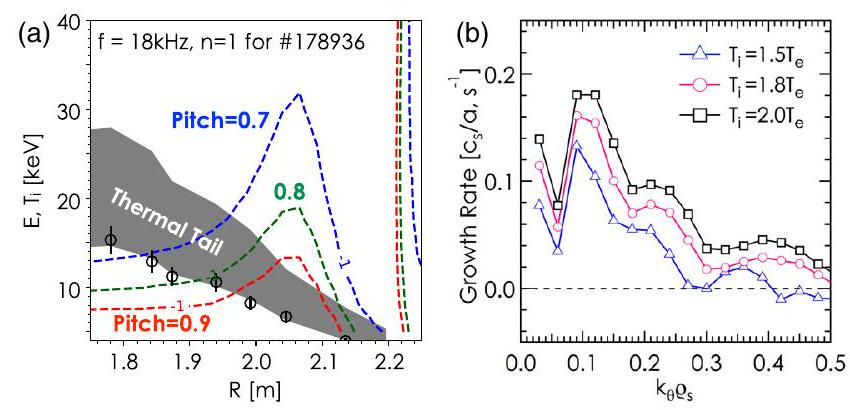
\includegraphics[max width=0.6\textwidth,max height=1.0\textheight]{2023_06_19_f8dbb752866ca158c73eg-5}
  	\caption{(a) The resonance lines in energy- $R$ space at the midplane for pitch 0.7 (blue), 0.8 (green), and 0.9 (red). The measured $T_{i}$ is represented by the circles and its high-energy thermal tail is indicated by the shaded band. (b) The growth rate (normalized by the ion sound speed, $c_{s}$ ) of AITG over a range of the $k_{\theta} \rho_{s}$ for fixed $\beta_{e}$, where $\rho_{s} \equiv\left(m_{i} T_{e}\right)^{0.5} / e B$. In experiment, $T_{i}$ is $1.8 T_{e}$ at the $q=1$ flux surface.}
  	\label{figure6}
  \end{figure}
  
  
 由于在高离子温度下模式会在理想MHDβ极限的一部分不稳定,并通过极快的场线重连和随机化导致小干扰,所以今后反应堆上它们的表现应该仔细研究,并在必要时发展缓解策略。
  
  \clearpage
  \section*{References}
  [1] W. Horton, D.-I. Choi, and W. M. Tang, Phys. Fluids 23, 590 (1980).
  
  [2] R. Nazikian, H. L. Berk, R. V. Budny, K. H. Burrell, E. J. Doyle, R. J. Fonck, N. N. Gorelenkov, C. Holcomb, G. J. Kramer, R. J. Jayakumar, R. J. La Haye, G. R. McKee, M. A. Makowski, W. A. Peebles, T. L. Rhodes, W. M. Solomon, E. J. Strait, M. A. VanZeeland, and L. Zeng, Phys. Rev. Lett. 96, 105006 (2006).
  
  [3] B. N. Breizman and S. E. Sharapov, Plasma Phys. Controlled Fusion 53, 054001 (2011).
  
  [4] F. Zonca, L. Chen, and R. A. Santoro, Plasma Phys. Controlled Fusion 38, 2011 (1996).
  
  [5] F. Zonca, L. Chen, R. A. Santoro, and J. Q. Dong, Plasma Phys. Controlled Fusion 40, 2009 (1998).
  
  [6] F. Zonca, L. Chen, J. Q. Dong, and R. A. Santoroc, Phys. Plasmas 6, 1917 (1999).
  
  [7] J. Candy, E. Belli, and R. Bravenec, J. Comput. Phys. 324, 73 (2016).
  
  [8] W. Chen et al., Europhys. Lett. 116, 45003 (2016).
  
  [9] P. B. Snyder et al., Nucl. Fusion 59, 086017 (2019).
  
  [10] R. J. Hawryluk, An empirical approach to tokamak transport, in Physics of Plasmas Close to Thermonuclear Conditions, edited by B. Coppi et al. (CEC, Brussels, 1980), Vol. 1, pp. 19-46.
  
  [11] B. A. Grierson, X. Yuan, M. Gorelenkova, S. Kaye, N. C. Logan, O. Meneghini, S. R. Haskey, J. Buchanan, M. Fitzgerald, S. P. Smith et al., Fusion Sci. Technol. 74, 101 (2018).
  
  [12] L. Chen, Phys. Plasmas 1, 1519 (1994).
  
  [13] A. Pankin, D. Mccune, R. Andre, G. Bateman, and A. Kritz, Comput. Phys. Commun. 159, 157 (2004).
  
  [14] H. L. Berk, B. N. Breizman, J. Candy, M. Pekker, and N. V. Petviashvili, Phys. Plasmas 6, 3102 (1999).
  
  [15] S. D. Pinches, I. T. Chapman, Ph. W. Lauber, H. J. C. Oliver, S. E. Sharapov, K. Shinohara, and K. Tani, Phys. Plasmas 22, 021807 (2015).
  
  [16] W. A. Peebles, T. L. Rhodes, J. C. Hillesheim, L. Zeng, and C. Wannberg, Rev. Sci. Instrum. 81, 10D902 (2010).
  
  [17] J. D. King, E. J. Strait, R. L. Boivin, D. Taussig, M. G. Watkins, J. M. Hanson et al., Rev. Sci. Instrum. 85, 083503 (2014).
  
  [18] A. M. Dimits et al., Nucl. Fusion 41, 1725 (2001).
  
  [19] R. H. Kraichhan, Phys. Fluids 10, 1417 (1967).
  
  [20] F. Zonca, L. Chen, S. Briguglio, G. Fogaccia, A. V. Milovanov, Z. Qiu, G. Vlad, and X. Wang, Plasma Phys. Controlled Fusion 57, 014024 (2015).
  
  [21] L. L. Lao, J. R. Ferron, R. J. Groebner, W. Howl, H. St. John, E. J. Strait, and T. S. Taylor, Nucl. Fusion 30, 1035 $(1990)$. [22] X. D. Du, M. W. Shafer, Q. M. Hu, T. E. Evans, E. J. Strait, S. Ohdachi, and Y. Suzuki, Phys. Plasmas 26, 042505 $(2019)$
  
  [23] Q. M. Hu, X. D. Du, Q. Yu, N. C. Logan, E. Kolemen, R. Nazikian, and Z. H. Jiang, Nucl. Fusion 59, 016005 (2019).
  
  [24] A. Bierwage, K. Shinohara, Y. Todo, N. Aiba, M. Ishikawa, G. Matsunaga, M. Takechi, and M. Yagi, Nat. Commun. 9, $3282(2018)$. [25] Z. Wang, Z. Lin, I. Holod, W. W. Heidbrink, B. Tobias, M. Van Zeeland, and M. E. Austin, Phys. Rev. Lett. 111, 145003 (2013).
  
  [26] E. Hirvijoki, A. Snicker, T. Korpilo, P. Lauber, E. Poli, M. Schneller, and T. Kurki-Suonio, Comput. Phys. Commun. 183, 2589 (2012).
  
  [27] I. Chavdarovski and F. Zonca, Phys. Plasmas 21, 052506 $(2014)$
  
  	%----------------------------------------------------------------------------------------
  \end{sloppypar}	
  \end{document}
